\clearpage
\section{New fitting: physical channels 5--8, 17 November 2026}
The owner fitted four CFD simulators on5--8, retained the RJ45 order
(slot7 ports0/1/2/3 to PM8/7/6/5), connected both USB pairs to8 and confirmed
all four shared monitor outputs connected to the SMU. Board DNA and MCU1803
were freshly verified. Qualified FPGA ff2f746c was restored to volatile SRAM;
no new build, MCU/CPLD/flash or clock-profile programming.
\subsection{Recorded coverage}
\begin{center}\begin{tabular}{rllllll}\toprule
Channel & ADC/bits & Integrator & TDC & Phase & Monitor & B/C/D\\\midrule
5 & NM/NM & NM & PASS & PASS & PASS & PASS\\
6 & NM/NM & NM & PASS & PASS & PASS & PASS\\
7 & NM/NM & NM & PASS & PASS & PASS & PASS\\
8 & PASS/PASS & PASS & PASS & PASS & PASS & PASS\\
\bottomrule\end{tabular}\end{center}
NM means not measured; INC means incomplete. USB remains on8, so no analog
coverage is inferred for5--7. PASS values are scoped functional tests, not a
whole-board release or traceable calibration.
\subsection{Channel8 ADC and integrators after USB correction}
Initial symptoms came from swapped USB pairs: DAC0/1 drove the driver path,
DAC2/3 the ADC bypass. Four active/inhibited-bypass probes identified the route.
The operator corrected the cables; the running exploratory scan was stopped with
native cleanup and excluded in full. Independent post-correction probes confirm
DAC0/1 at J8, DAC2/3 at J6 and normal selector map[0,1].
The apparent bank inversion and lower driver-path gain are not ADC defects.

Only post-correction data enter selected results: both257-point ADC sweeps span
-1.2 to+1.2V at1V common mode (legs0.4--1.6V); every bit and all44adjacent-pair
states are exercised. Earlier driver-path and insufficient/wider-range attempts
remain archived as diagnostics, not qualification evidence.
\begin{center}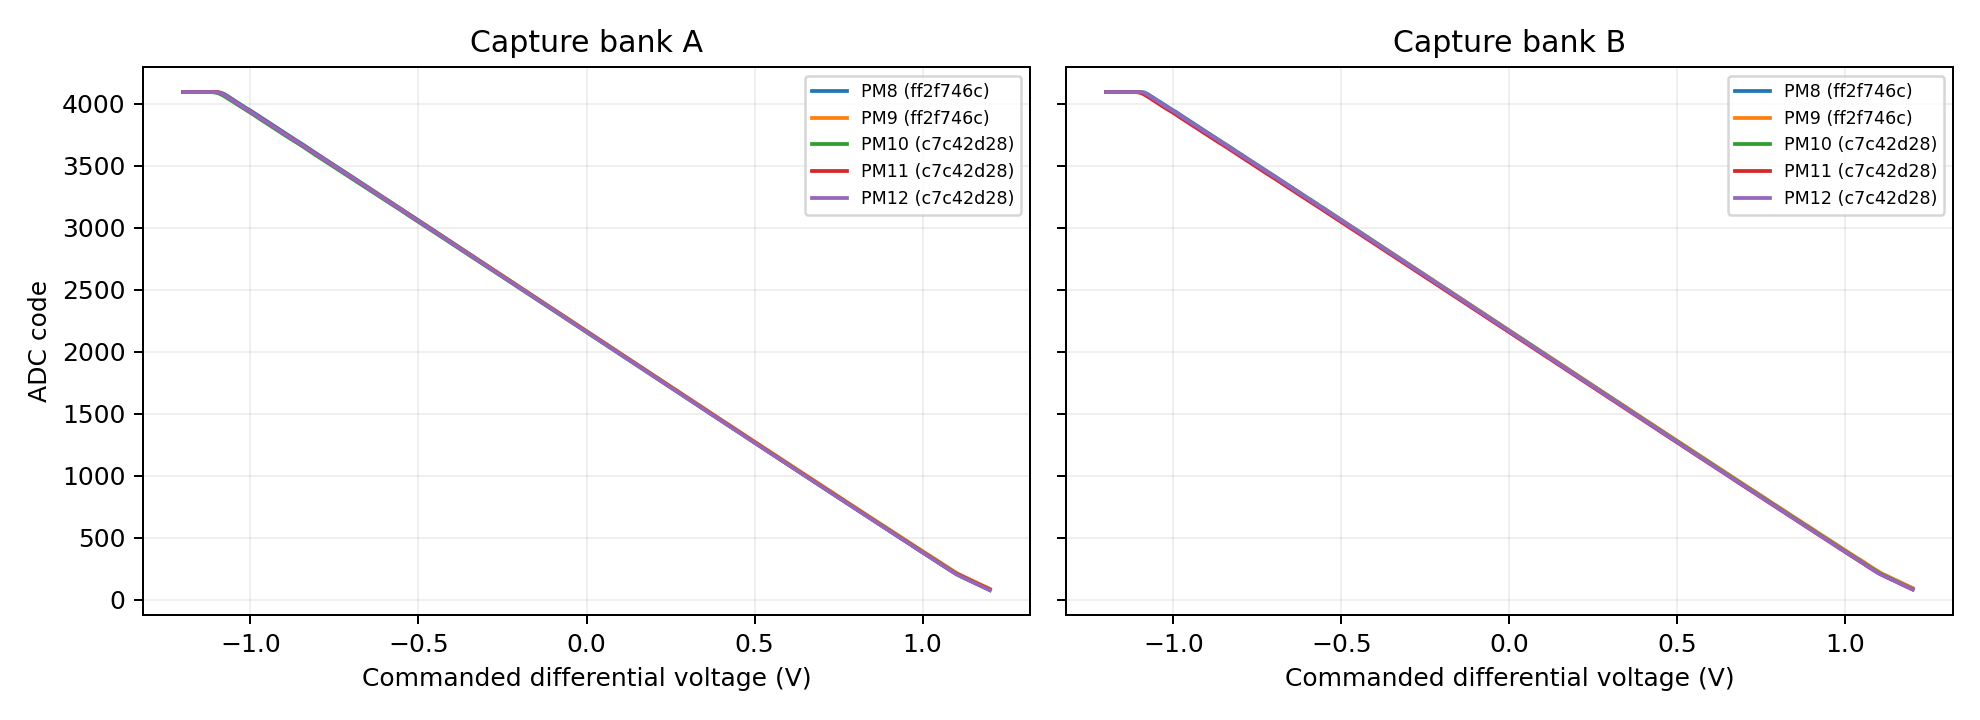
\includegraphics[width=\linewidth]{group58-adc-response-08-12.png}\end{center}
Historical10--12 use c7c42d28,9 and8 use ff2f746c with their respective frozen
source contracts. Axes show commanded voltages and complete-chain response,
not calibrated ADC-only gain or input voltage.

The selected integrator scan uses corrected DAC2/3 routing and the original
1.024/2.048V base coordinate: coarse13points, fine26points at0.4mV, independent
candidate revisits and plus/minus5mV controls. Clipped or ambiguous traces are
excluded. Earlier all-zero traces came from the disconnected bypass stimulus;
they do not constitute an integrator hardware failure.
\begin{center}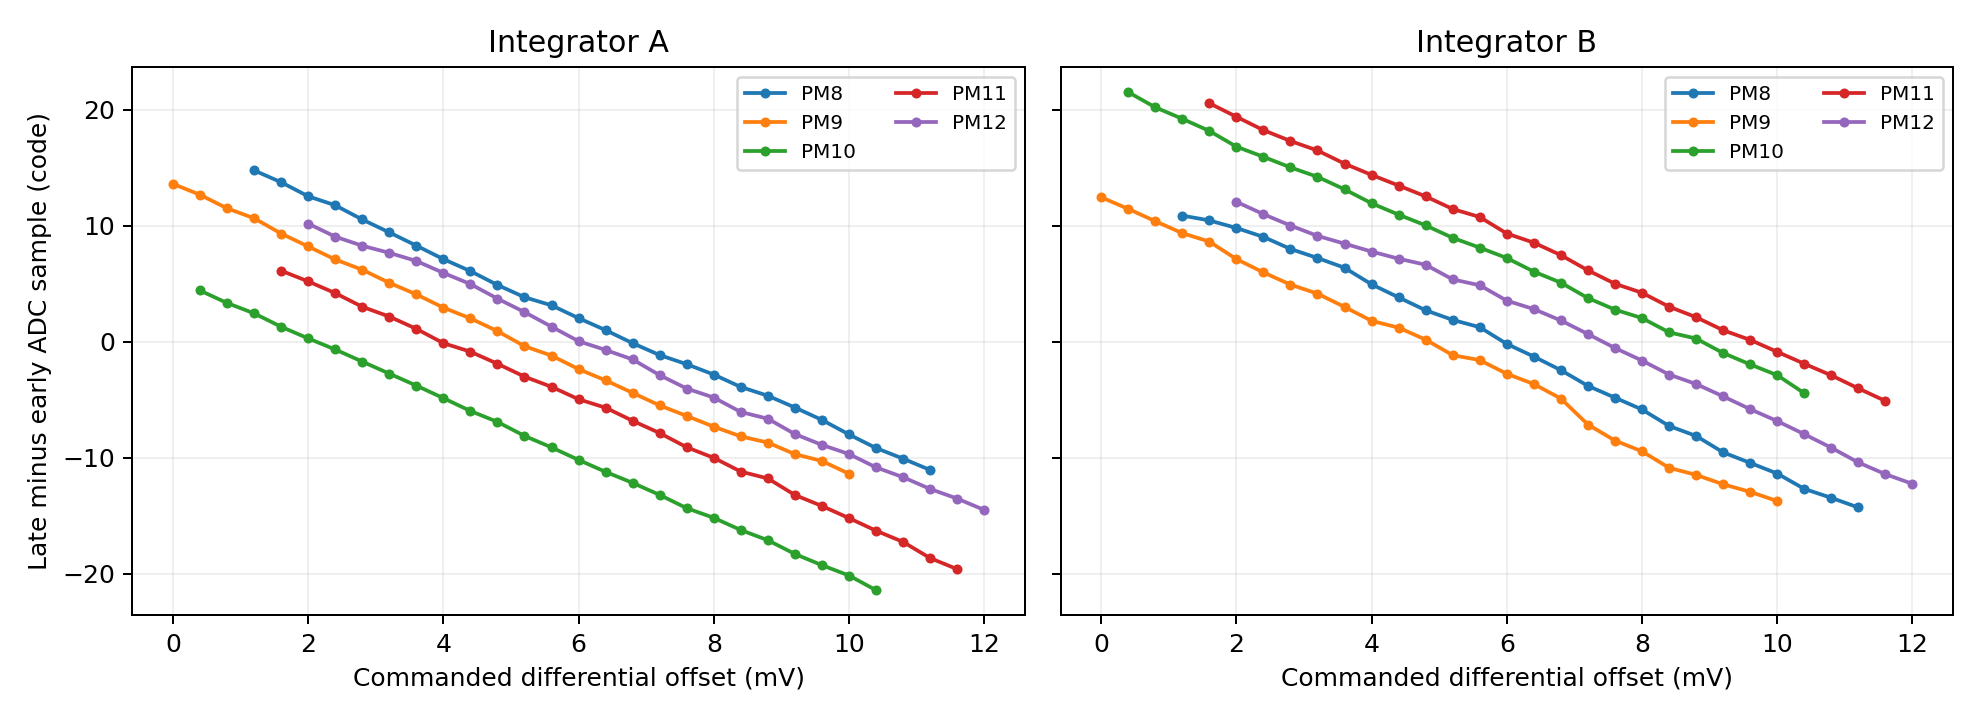
\includegraphics[width=\linewidth]{group58-integrator-response-08-12.png}\end{center}
\subsection{Zero-input waveforms and spectra}
These overlays use only explicitly selected PASS receipts from physical8--12.
Zero differential input is commanded at1V on both direct-stimulus outputs.
Waveforms retain the raw four-phase structure; local capture origins are not
phase aligned. The one-sided RMS spectrum is in ADC codes per bin, not noise
density. Frequency/time axes assume80.1574MS/s. These whole-chain observations
do not estimate intrinsic ADC noise or aperture jitter.
\begin{center}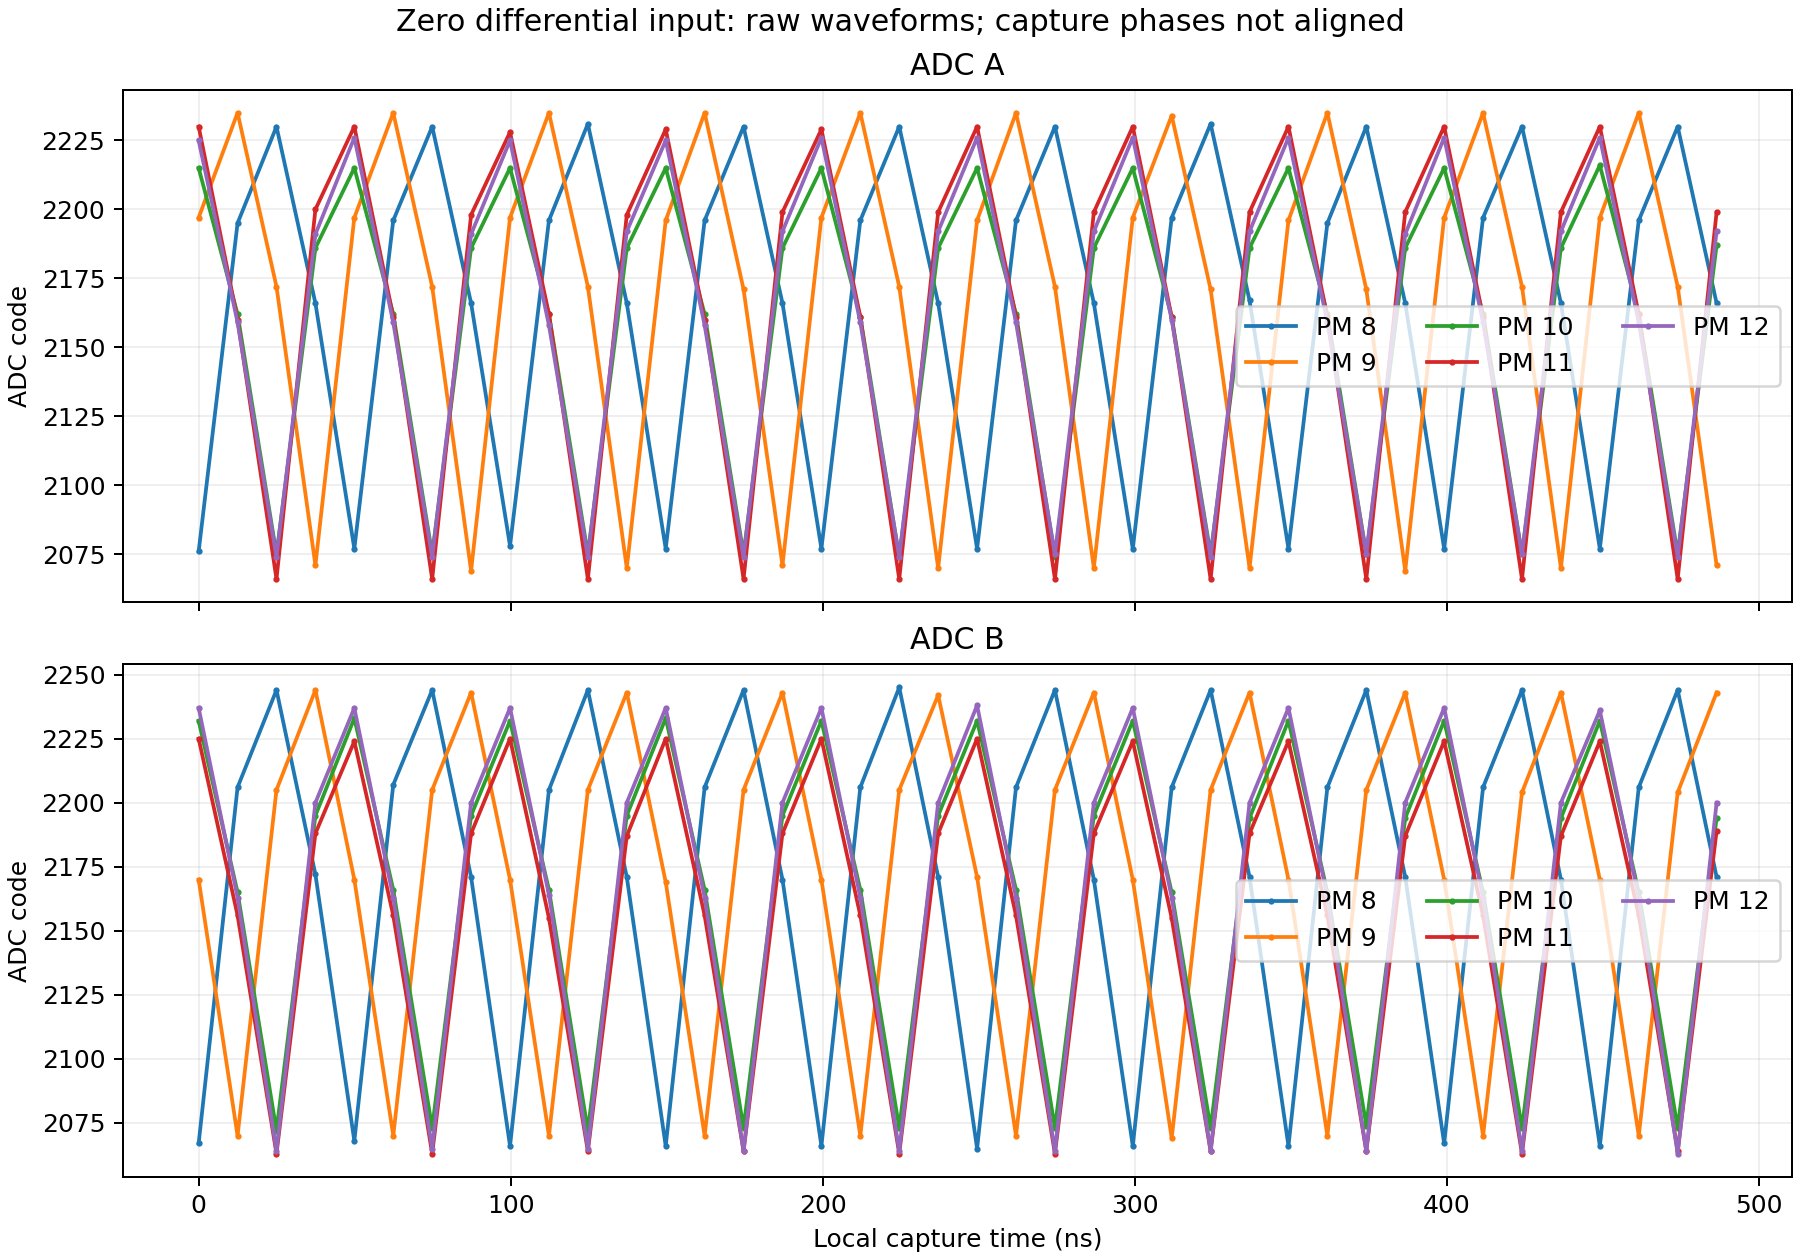
\includegraphics[width=\linewidth]{group58-adc-zero-time.png}\end{center}
\begin{center}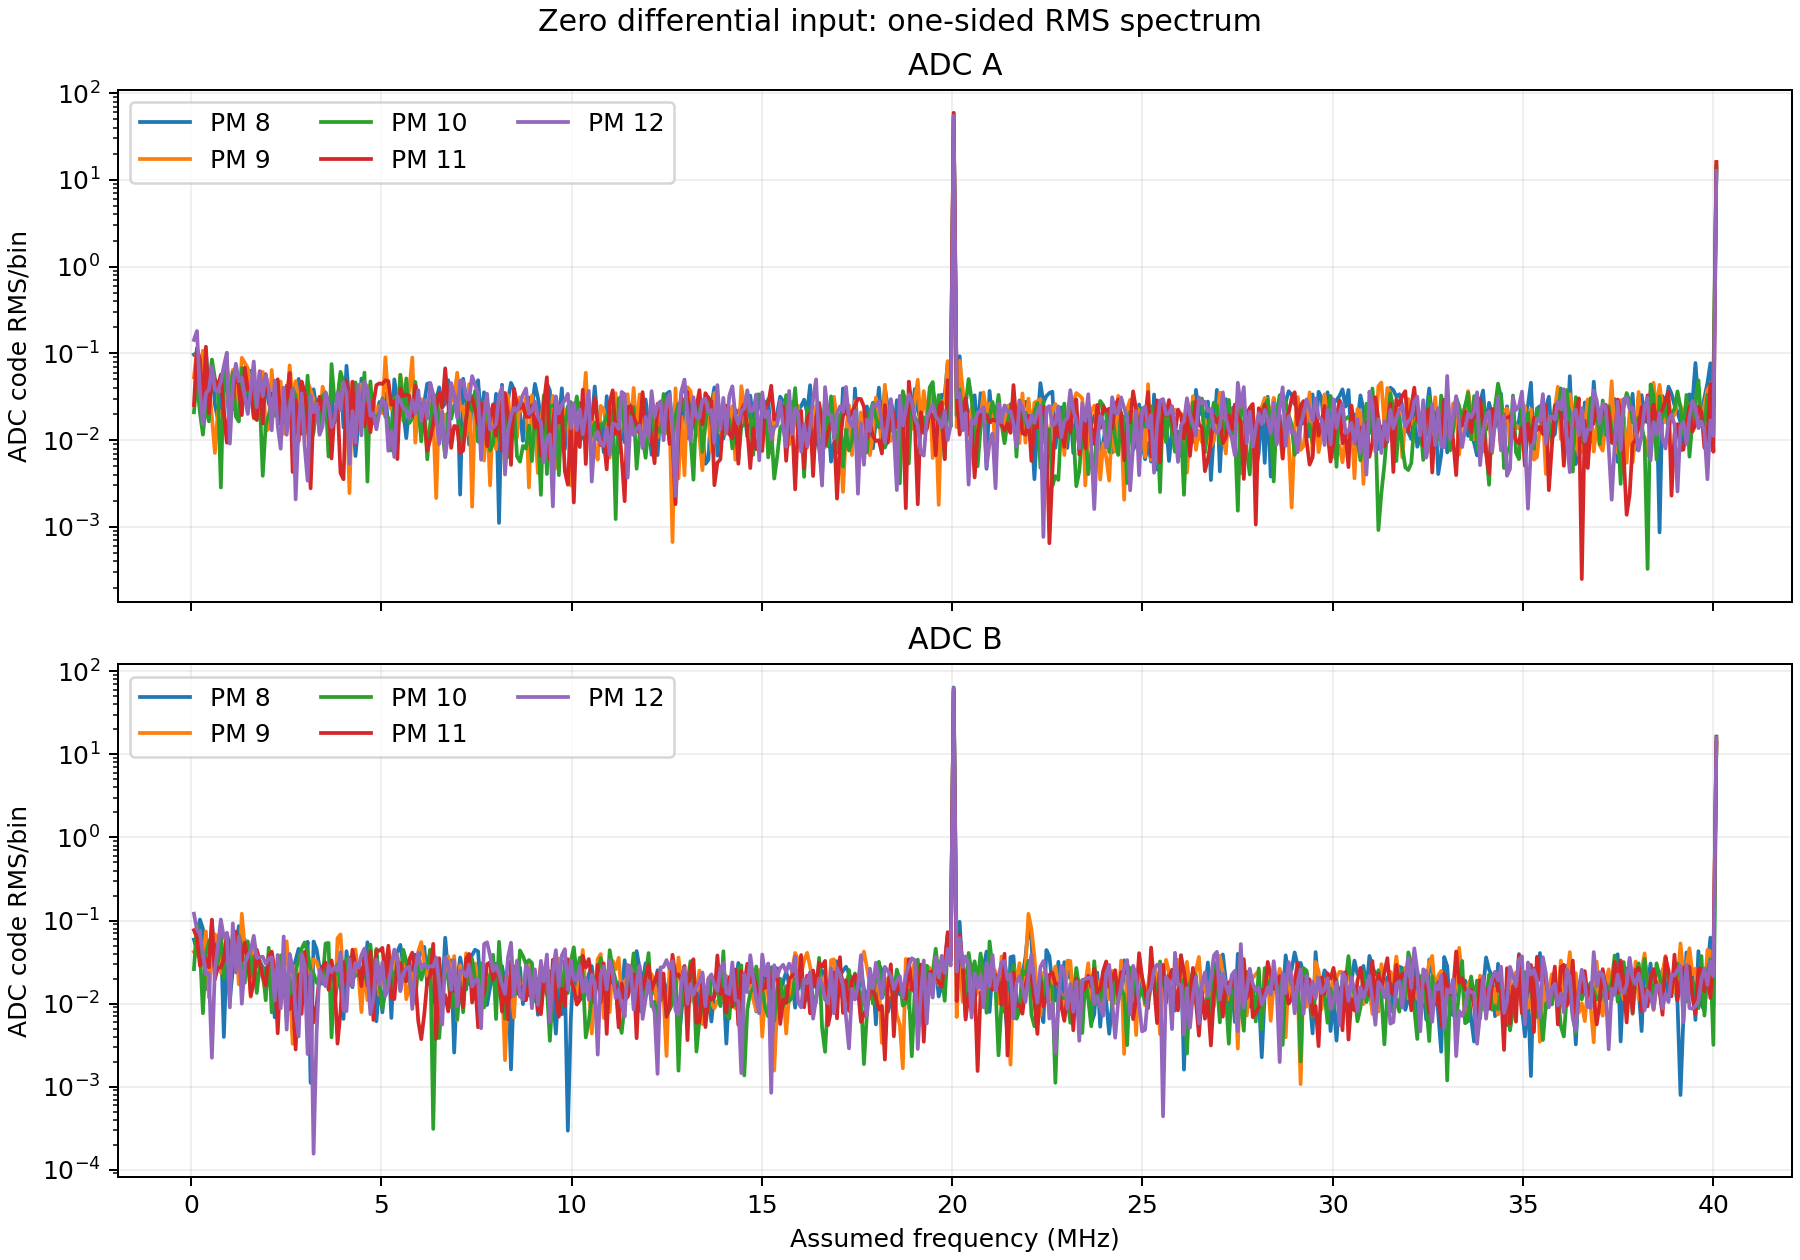
\includegraphics[width=\linewidth]{group58-adc-zero-fft.png}\end{center}
\subsection{Finite TDC patterns and gate-phase scans}
The clock40 acquisition includes discovery, quiet controls, count1/64/512/1024
and25phase positions per port. All raw13-bit words and count conservation are
independently checked. Phase is relative to nominal serializer slots; no absolute
TDC calibration or intrinsic jitter measurement is claimed. Historical9--12
TDC curves use the corrected-clock c7531465 captures from14November; withdrawn
c7 TDC curves are not used. Other historical overlays retain their dated
acquisition conditions and do not imply a fresh retest of9--12.
\begin{center}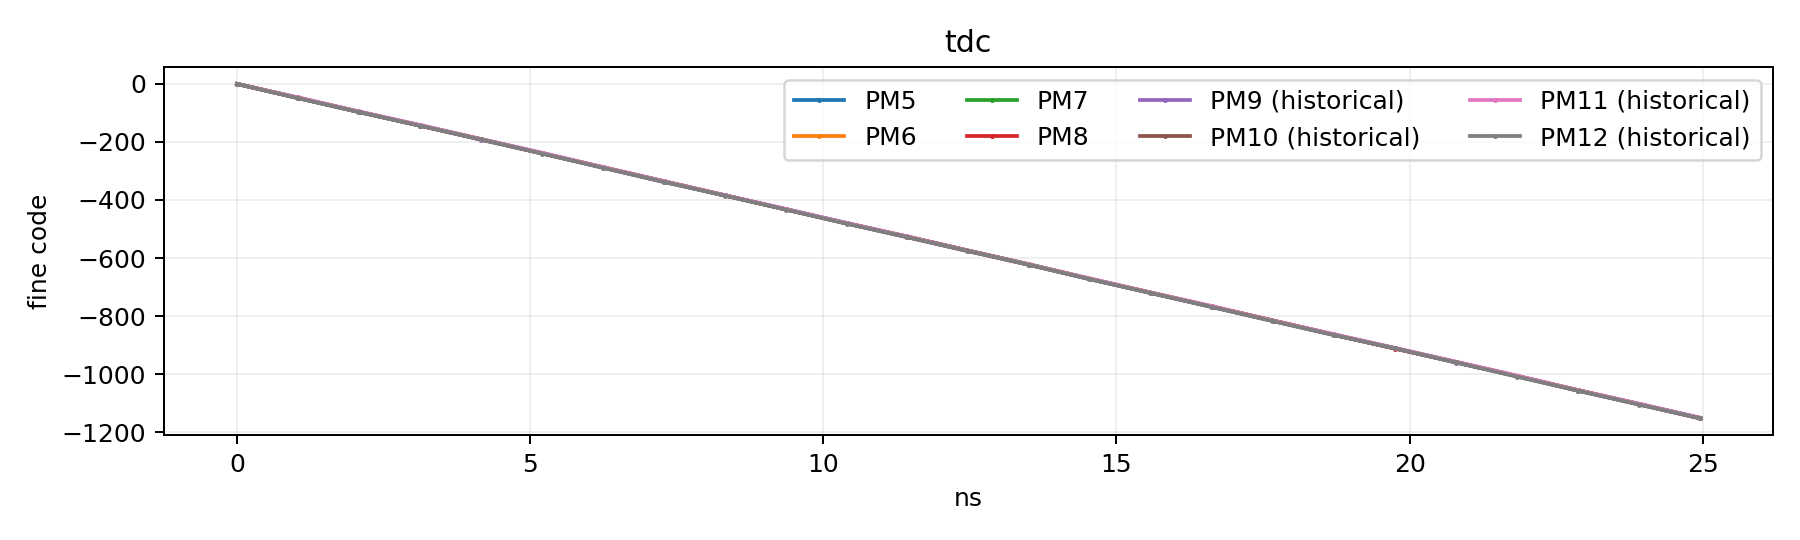
\includegraphics[width=\linewidth]{group58-tdc-05-08.png}\end{center}
\begin{center}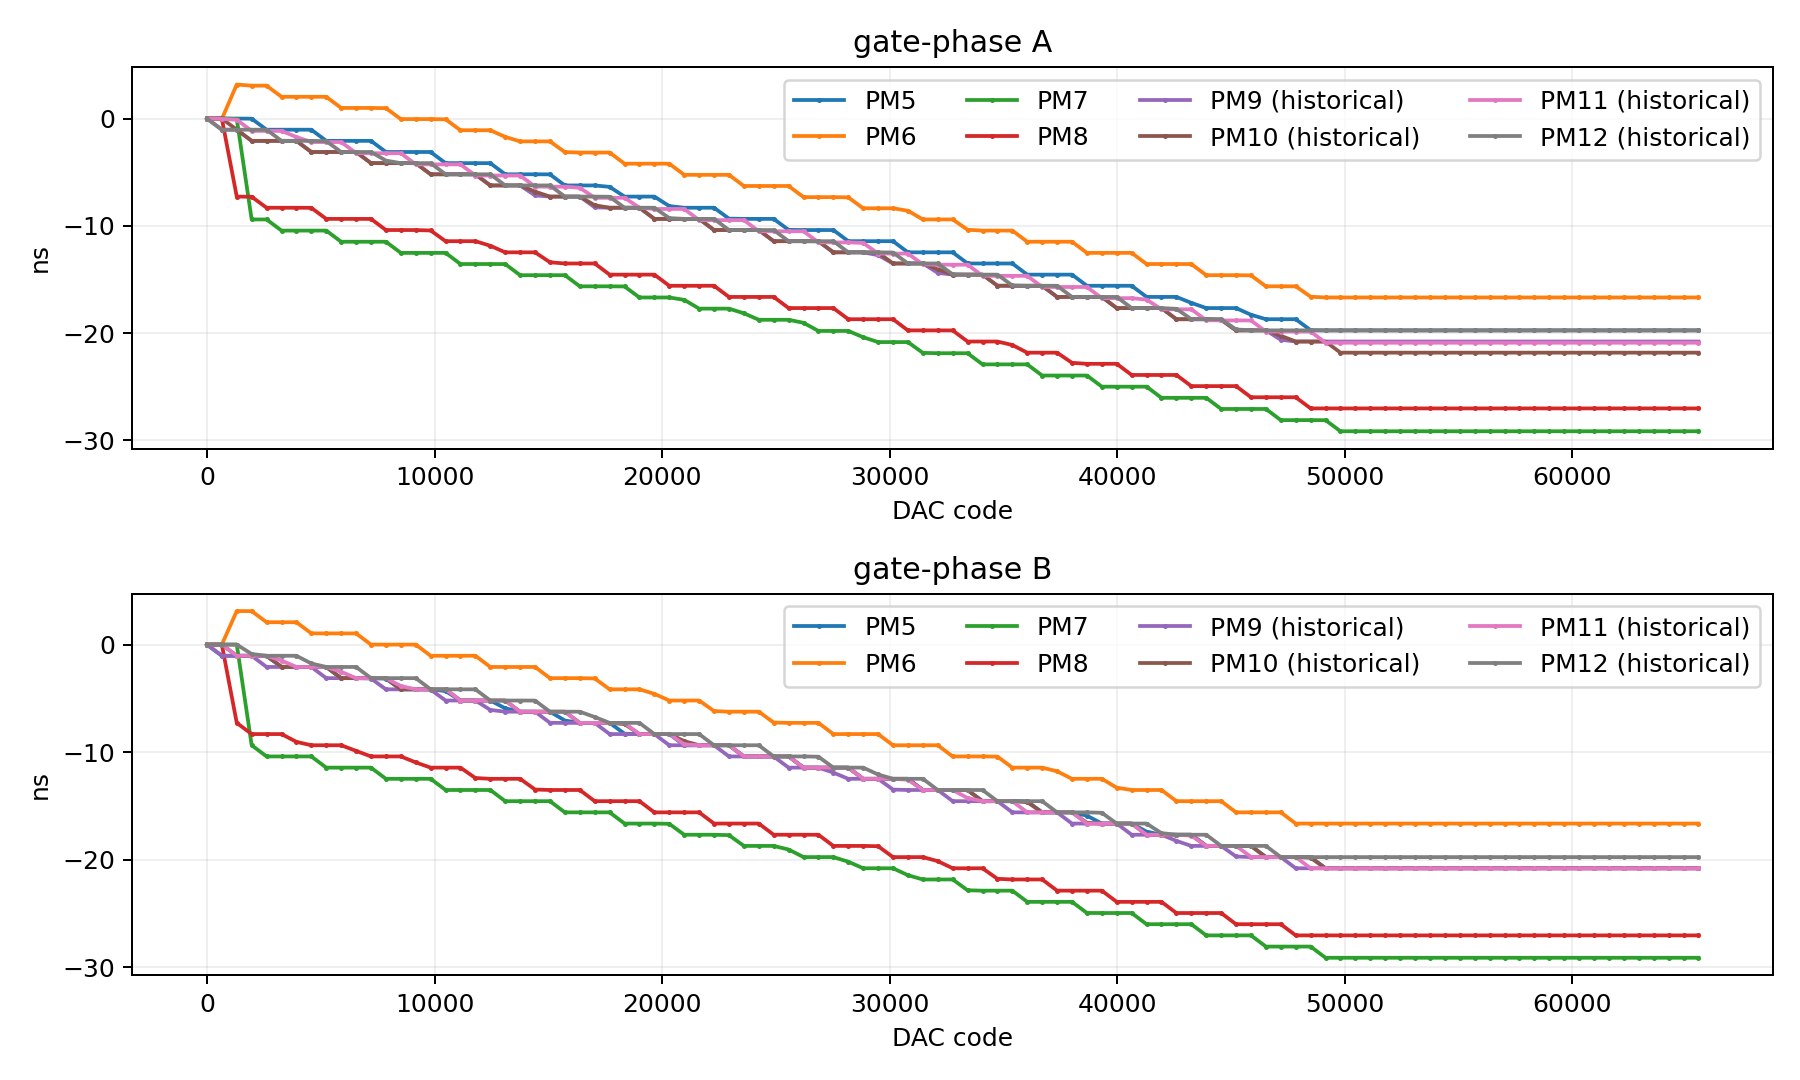
\includegraphics[width=\linewidth]{group58-gate-phase-05-08.png}\end{center}
Gate phase uses101DAC-A codes per channel and both sampled return lanes.
Nearest-continuation unwrap retains discontinuities; a functional excursion
is not a certified smooth tuning range or sub-bin accuracy.
\subsection{Shared SMU measurements}
Eight monitor inputs and three101-code DAC curves per module were read with
Keysight B2910BL as0A/local Force HI/LO voltmeter. Only one shared mux was
active at a time. Negative/positive supply divider values use nominal53/33.
\begin{center}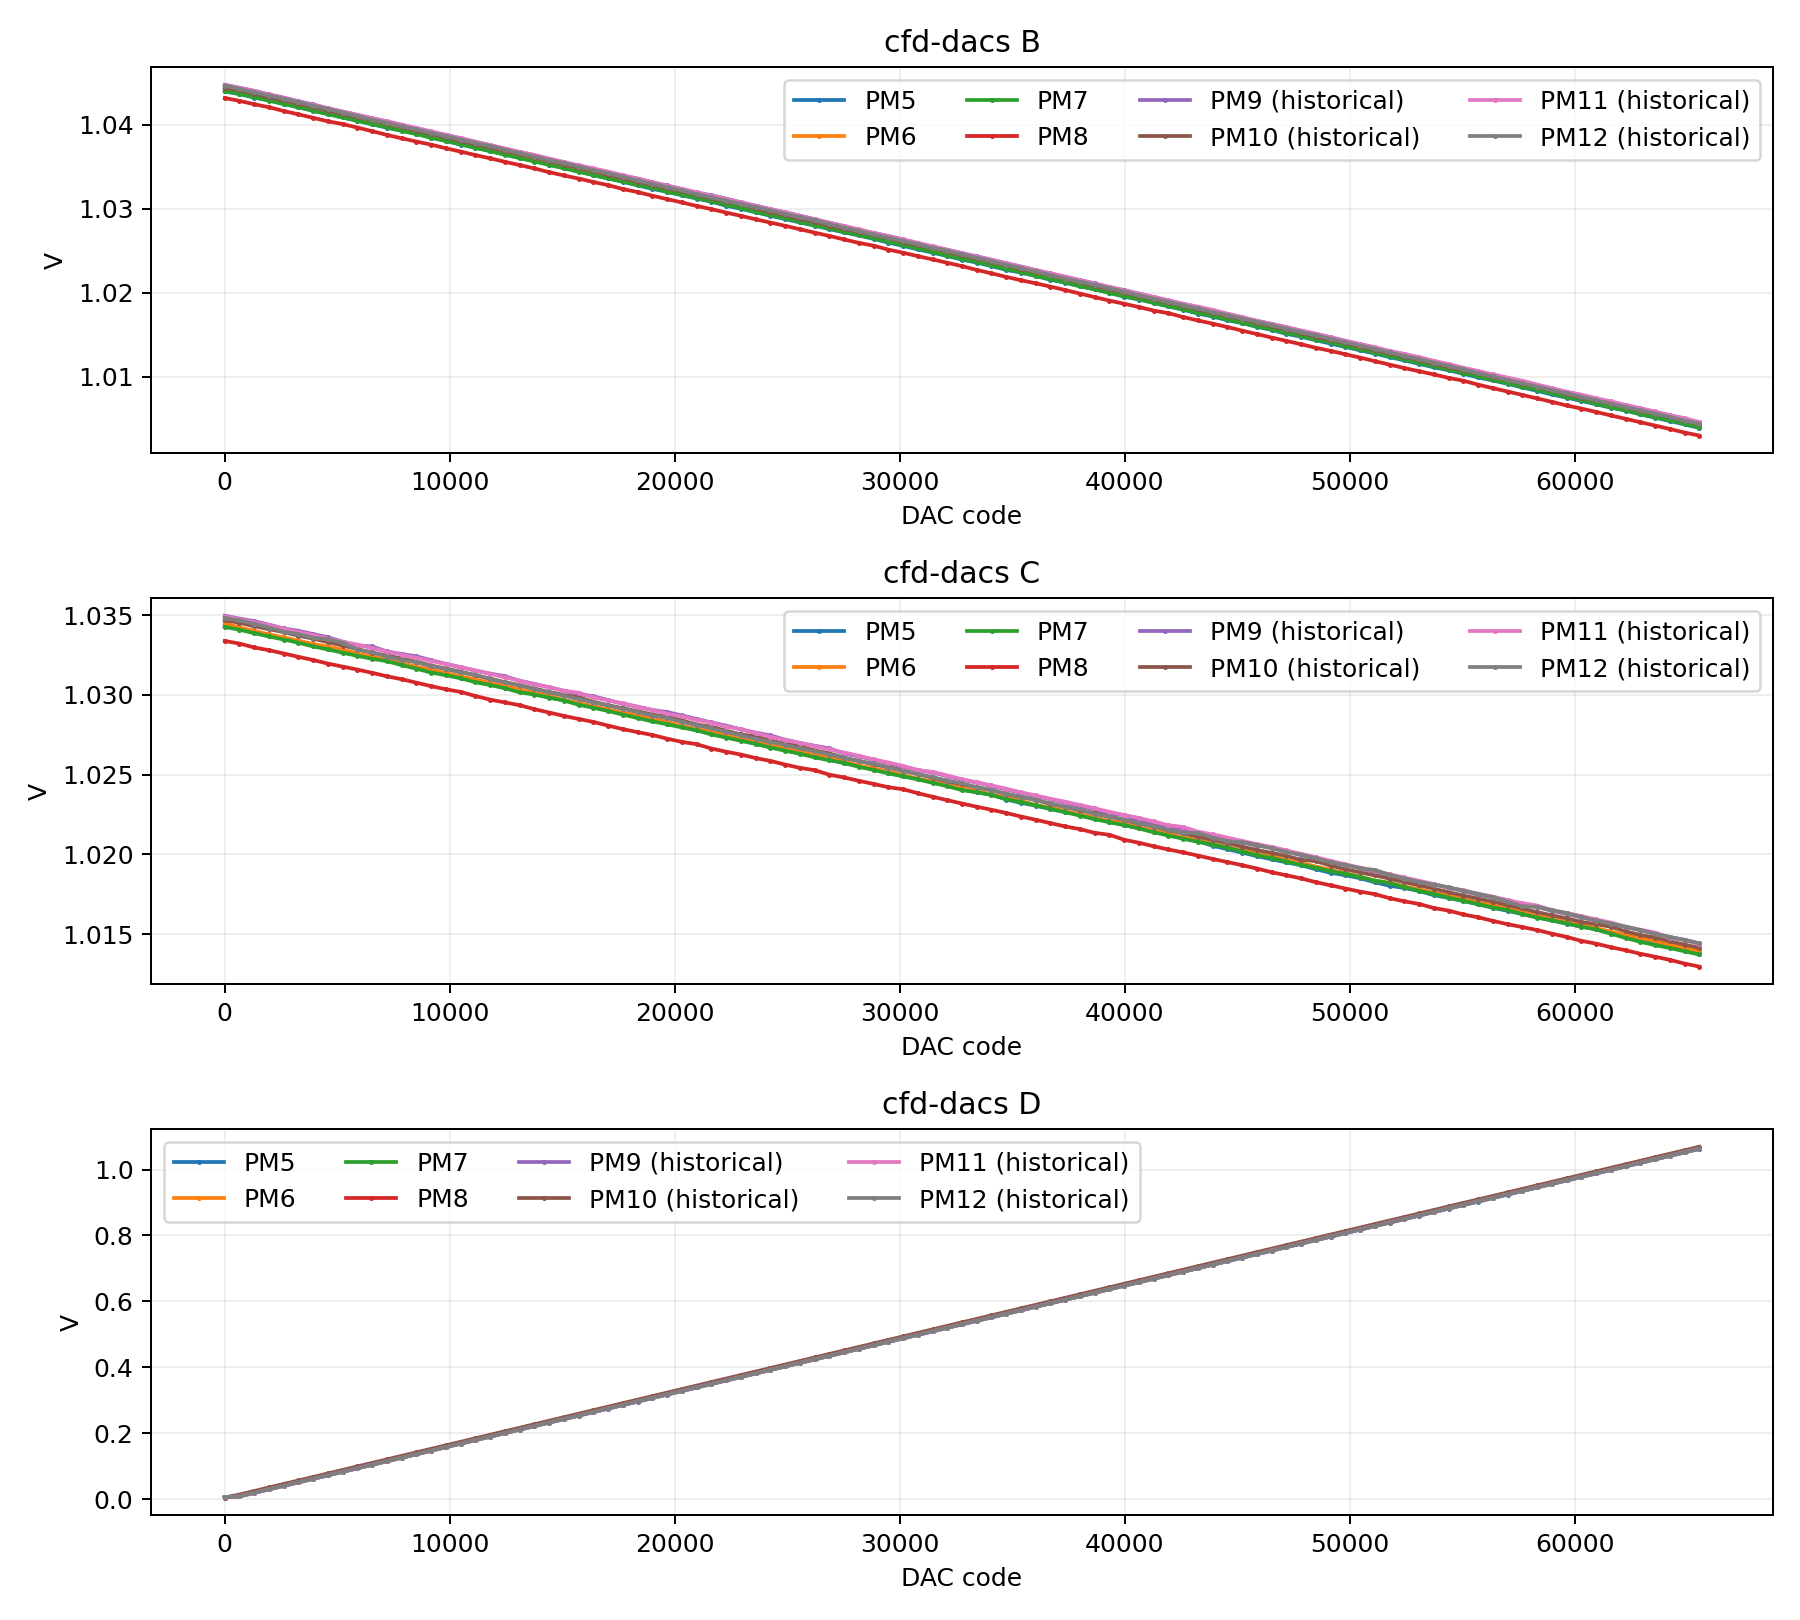
\includegraphics[width=\linewidth]{group58-cfd-dacs-05-08.png}\end{center}
Final SMU OFF/HIZ/0A, auto-on disabled; all four monitor muxes inhibited and
TCA masks zero. Exercised B/C/D and phase DAC-A restored to0000. Kasli HDMI
SPI outputs remain driven; no global stop or slot6 direction change.
All original data and selected historical cases are preserved. Raw campaign,
source snapshots and independent validation receipts are in the dated group5--8
archive; this chapter is editable LaTeX.
